%設定頁面
\documentclass[12pt,a4paper]{article}
\usepackage[margin=1in,a4paper]{geometry}

%設定中文
\usepackage{xeCJK} 
\setCJKmainfont{標楷體} 
\XeTeXlinebreaklocale "zh"   
\XeTeXlinebreakskip = 0pt plus 1pt 

%浮水印
%\usepackage{draftwatermark}
%\SetWatermarkText{\bf NTNU MATH}
%\SetWatermarkScale{0.7}

%圖片
\usepackage{graphicx}
\usepackage{subfigure}

%頁首頁尾
\makeatother
\usepackage{fancyhdr}

%顏色
\usepackage{xcolor}

%表格顏色
\usepackage{colortbl}

%設定數學
\usepackage{amsmath, amsthm, amssymb}
\makeatletter

%自定圈圈標號
\usepackage{pstricks,pstricks-add}
\newcommand\textc[1]{{\begin{pspicture*}
(-0.25,-0.2)(0.25,0.3)\rput[c](0,0)
{\large \textcircled{\footnotesize #1}}
\end{pspicture*} }}

%自訂向量符號
\def\leftharpoonfill@{\arrowfill@\leftharpoonup\relbar\relbar}
\def\rightharpoonfill@{\arrowfill@\relbar\relbar\rightharpoonup}
\newcommand\rbjt{\mathpalette{\overarrow@\rightharpoonfill@}}
\newcommand\lbjt{\mathpalette{\overarrow@\leftharpoonfill@}}

%自訂定理
\newtheorem*{thm}{Theorem}
\newtheorem*{lem}{Lemma}
\newtheorem*{de}{Definition}
\newtheorem*{rmk}{Remark}
\newtheorem*{ex}{Example}
\newtheorem*{pf}{Proof}
\newtheorem*{sol}{Solution}

%程式碼
\usepackage{listings}
\usepackage{color}

\definecolor{dkgreen}{rgb}{0,0.6,0}
\definecolor{gray}{rgb}{0.5,0.5,0.5}
\definecolor{mauve}{rgb}{0.58,0,0.82}

\lstset{
  basicstyle={\small \ttfamily},
  frame=tb,
  language=Python,
  aboveskip=3mm,
  belowskip=3mm,
  showstringspaces=false,
  columns=flexible,
  basicstyle={\small\ttfamily},
  numbers=left,
  numbersep = 14pt,
  numberstyle=\tiny\color{gray},
  keywordstyle=\color{blue},
  commentstyle=\color{dkgreen},
  stringstyle=\color{mauve},
  breaklines=true,
  breakatwhitespace=true,
  tabsize=3,
  backgroundcolor=\color{gray!10}
}




%作者
\title{NTNU影像處理HW3}
\author{廖家緯}
\date{2020.3.31}

\begin{document}
\maketitle
%標題、作者、日期
\fontsize{12pt}{20pt}\selectfont
%設定字體大小、間距
\setlength{\baselineskip}{20pt}
%設定行距

\pagestyle{fancy}
\lhead{}
\chead{}
\rhead{}
\lfoot{}
\cfoot{\thepage}
\rfoot{}
\renewcommand{\headrulewidth}{0pt} %上線寬
\renewcommand{\footrulewidth}{0pt} %下線寬
%\renewcommand{\abstractname}{Executive Summary}




%正文開始
\begin{enumerate}
\item[•]{\bf Outline}:
For each pixel $I(x,y)$,
\begin{enumerate}
\item[1)]Calculate quantization error
\vspace*{1em}\\
$E(x,y)=
I(x,y) = \begin{cases}
I(x,y), & \text{if } I(i,j)<128\\
I(x,y)-255, & \text{if } I(i,j)\geq 128
\end{cases}$.
\vspace*{1em}\\

\item[2)]
Spread the error according to Floyd-Steinberg\\
i.e.,
\begin{center}
$\begin{array}{|c|c|c|}
\hline
 & \cellcolor{gray!20}(x,y) & +\frac{7}{16}E\\
\hline
+\frac{3}{16}E & +\frac{5}{16}E & +\frac{1}{16}E\\
\hline
\end{array}$
\vspace*{2em}\\
\end{center}

\item[3)]
Quantize new $I(x,y)$ to 0 or 255 using 128 as the threshold
\vspace*{2em}\\
\end{enumerate}


\item[•]
{\bf Code(Python):}
\begin{lstlisting}
# coding: utf-8

#引入模組
import numpy as np
import cv2

# 讀取灰階影像
I = cv2.imread('Gray.jpg', cv2.IMREAD_GRAYSCALE)

#判斷影像的矩陣大小
n = np.shape(I)[0]
m = np.shape(I)[1]
E = np.zeros((n,m), np.double)
I = np.double(I)

#For each pixel I(x,y)
for i in range(n):
    for j in range(m):
        
        #1)Calculate quantization error
        if I[i, j] >= 128:
            E[i, j] = I[i, j]-255
        else:
            E[i, j] = I[i, j]
            
        #2)Floyd-Steinberg    
        if j+1<=m-1:
            I[i, j+1] += (7/16)*E[i, j]
        if i+1<=n-1 and j-1>=0:
            I[i+1, j-1] += (3/16)*E[i, j]
        if i+1<=n-1:
            I[i+1, j] += (5/16)*E[i, j]
        if i+1<=n-1 and j+1<=m-1:
            I[i+1, j+1] += (1/16)*E[i, j]

#3)Quantize new I(x,y) to 0 or 255 using 128 as the threshold
for i in range(n):
    for j in range(m):
        if I[i, j]>=128:
            I[i, j] = 1
        else:
            I[i, j] = 0
I = I*255           
I = np.uint8(I)

\end{lstlisting}

\item[•]
{\bf Result:}
\begin{figure}[h]
\hspace*{3em}
\begin{tabular}{cc}
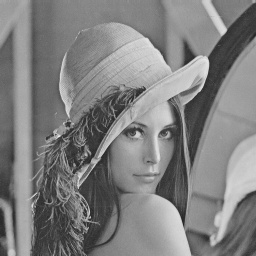
\includegraphics[height=2.4in]{Gray.jpg}&
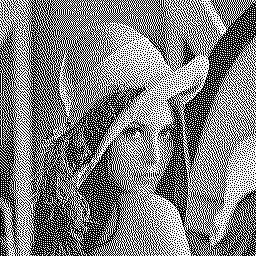
\includegraphics[height=2.4in]{Floyd-Steinberg.jpg}\\
原圖  & Floyd-Steinberg
\end{tabular}
\end{figure} 

\newpage
\item[•]
{\bf Experience:}\\
這次作業花了很多時間debug。最初我誤解老師題目的意思,我先將$E$矩陣建完後才去更新每個$I$矩陣,也就是分別用兩個雙重迴圈完成$E$和$I$,然而做出來的結果非常怪異,因此我反覆重看老師的題目後,才發現兩件事情要在同一個迴圈做。而第二個令我困擾的問題是我一開始忘了將$I$轉型,導致我做出來的碎片感很重,事實上我對各種的型態還不太熟(沒修過資工的計概),所以只能上網查資料,一個一個嘗試,花我不少的功夫才完成。另外,這次的作業可以明顯感覺我的方法需要跑大約3到5秒的時間,雙重迴圈(O($n^2$))的時間複雜度讓程式執行的時間上升許多,之後我想嘗試用一些矩陣計算的技巧進行優化,降低程式執行的時間複雜度。
\end{enumerate}










\end{document}